\apendice{Documentación de usuario}

\section{Introducción}
En este apartado se comenta una parte esencial dentro de la documentación de un proyecto, los manuales de usuario. Estos son documentos donde los desarrolladores tienen que poner toda la información necesaria para instalar y ejecutar los programas y/o aplicaciones que han desarrollado. Estos documentos tienen que tener también los requisitos que se necesitan para poder instalar y ejecutar los programas, e incluso pueden incluir comentarios que nos dicen que hacer en caso de error de la aplicación.

Este apartado ha sido dividido por los distintos manuales de las distintas aplicaciones que he hecho, de cada una se comentarán los requisitos de los usuarios, la instalación y como se ejecuta. Estas aplicaciones de las que vamos a hablar son:
\begin{itemize}
	\item \textbf{Aplicación de grabación prototipo:} aplicación que un principio iba a ser la aplicación con la cual generar datos. Nos permite grabar audios con el nombre que elijamos.
	\item \textbf{Aplicación para la recogida de datos:} aplicación final para la recogida que nos permite grabar un audio y seleccionar tanto las opciones adicionales como las emociones o respuesta relacionada.
	\item \textbf{Aplicación para la interpretación:} aplicación final AVC que nos permite modificar las opciones adicionales de los pacientes comunes a todos los dispositivos y nos permite interpretar una emoción o una respuesta.
\end{itemize}
\section{Aplicación de grabación prototipo}
\subsection{Uso}
Este es un prototipo de la aplicación final, en este prototipo se permite grabar y dar nombre a audios y reproducirlos.

Estos audios se almacenan en un carpeta llamada Apace localizada en la raíz.

\subsection{Requisitos}
El requisito principal es contar con un dispositivo \textit{smartphone Android} actualizado, con versión \textit{Android} 6.0 o superior.

\subsubsection{Instalación}
Para poder instalar la aplicación el único requisito que se necesita es conexión a Internet para poder descargarse la aplicación.

\subsubsection{Ejecución}
Para la ejecución del prototipo solo se requiere que la aplicación esté instalada y que se acepten los permisos de grabación de audio y de escritura que se preguntan al principio de la ejecución.

\subsection{Instalación}
La instalación del prototipo es sencilla, solo hay que descargar el archivo \textit{apk} desde donde se haya sido suministrado (correo, \textit{WhatsApp}, \textit{GitHub}) y realizar los ajustes necesarios para poder descargarla al ser una aplicación ajena a \textit{Play Store}.

Estos ajustes adicionales consisten simplemente aceptar que se descargue esta aplicación exterior a \textit{Play Store}.

Una vez descargada el \textit{apk} de la aplicación aparecerá en su menú de aplicaciones instaladas con el nombre de Apace, como se puede ver en la figura~\ref{fig:logopro}.

\begin{figure}[htp]
	\centering
	
\includegraphics[scale=0.6]{logopro}
	\caption{Logotipo y nombre de la aplicación una vez instalada.}
	\label{fig:logopro}
\end{figure}

\subsection{Ejecución}
Para la ejecución solo tenemos que pulsar el logotipo anteriormente mostrado. En la primera ejecución que hagamos del prototipo nos saldrá el siguiente diálogo, para pedirnos permisos para poder usar tanto el sistema de grabación de audio, como para poder almacenar archivos. Debemos dar permisos a ambos pulsando en la opción \textit{Permitir}. Es muy importante aceptar estos permisos ya que sino la aplicación se cerrará en la primera vez que queramos grabar un audio. En cualquier caso si por algún error se ha denegado los permisos y la aplicación se ha cerrado se puede volver a abrir y nos volverá a pedir aceptar los permisos. La petición de estos permisos se pueden ver en las figuras~\ref{fig:properr1} y ~\ref{fig:proper2}.

\begin{figure}[htp]
	\centering
	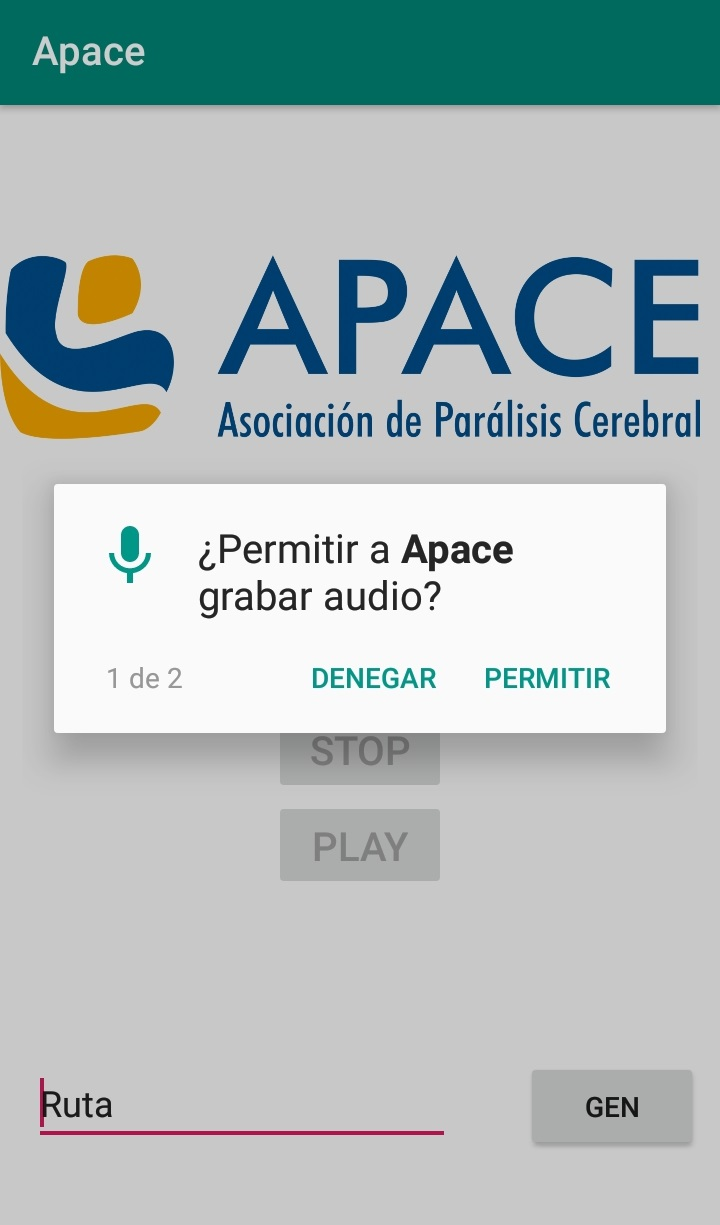
\includegraphics[scale=0.3]{proper1}
	\caption{Petición de permisos para la grabación de audio.}
	\label{fig:properr1}
\end{figure}

\begin{figure}[htp]
	\centering
	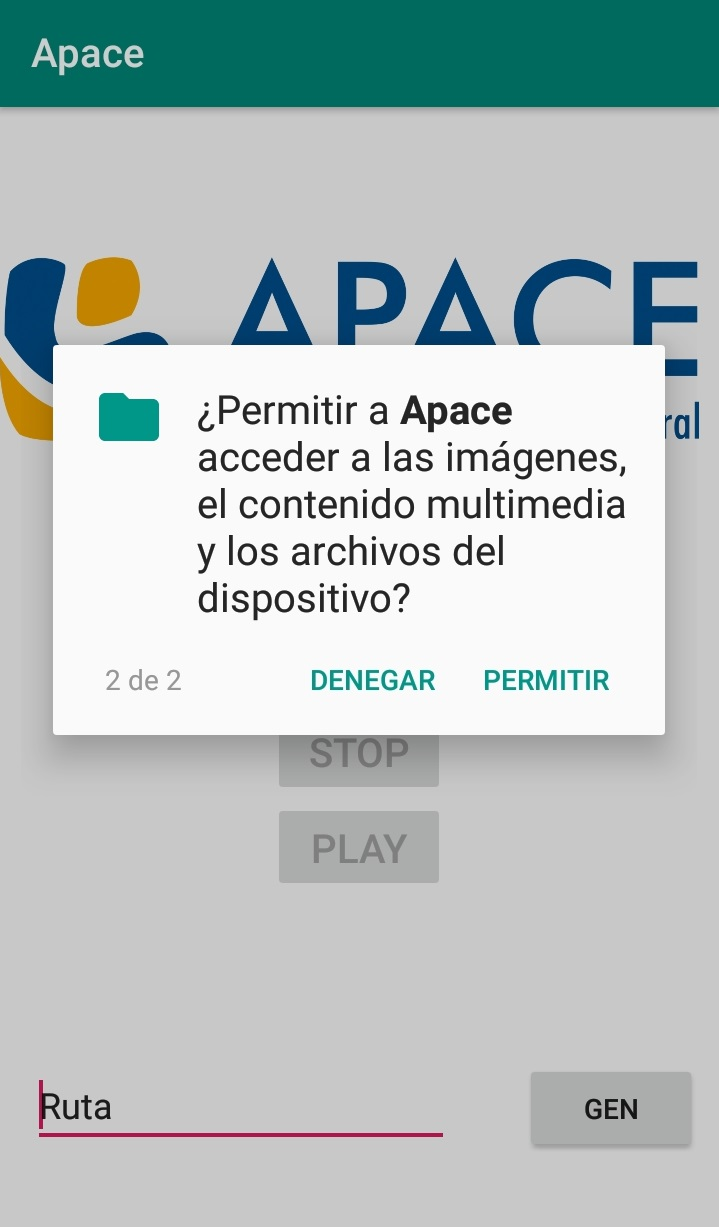
\includegraphics[scale=0.3]{proper2}
	\caption{Petición de permisos para el acceso al almacenamiento multimedia.}
	\label{fig:proper2}
\end{figure}

Después de aceptar los permisos tendremos acceso al menú principal de la aplicación, como se ve en la figura~\ref{fig:promp}, en el se pueden ver 3 botones (\textit{RECORD}, \textit{STOP} y \textit{PLAY}) y una caja de texto con un botón \textit{GEN}.

\begin{figure}[htp]
	\centering
	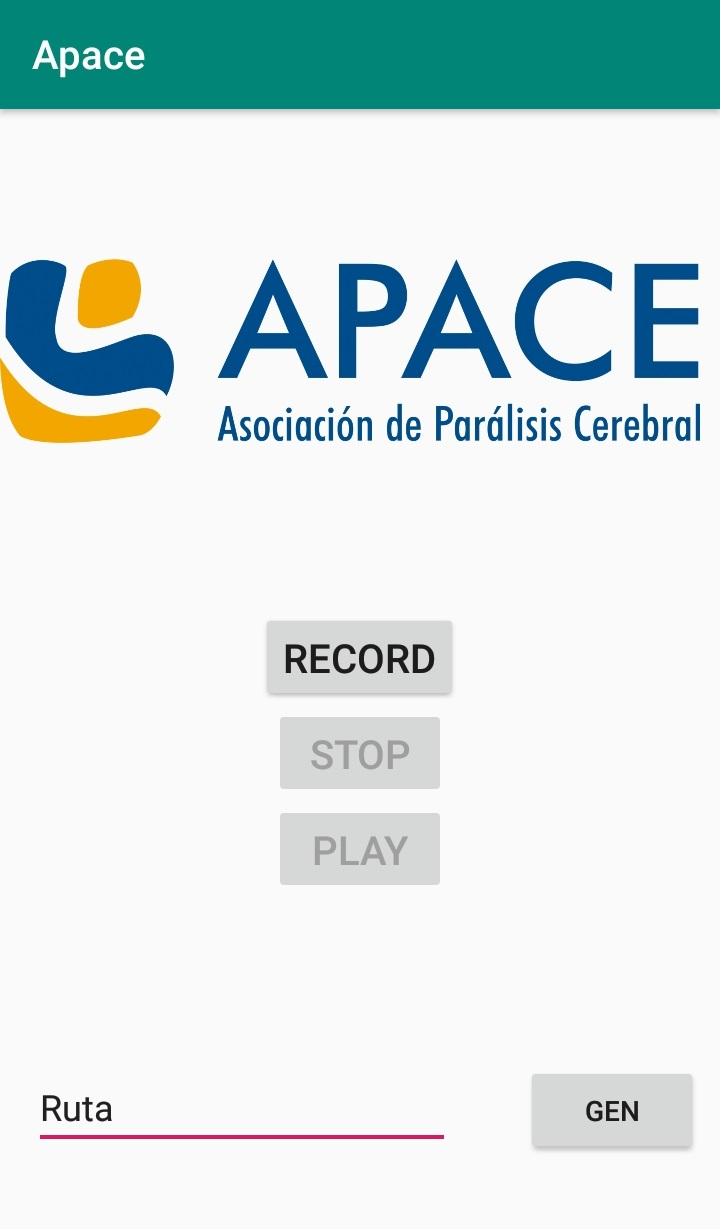
\includegraphics[scale=0.3]{promp}
	\caption{Menú principal de la aplicación prototipo.}
	\label{fig:promp}
\end{figure}

Los tres primeros botones sirven para manejar la grabación de los audios, al principio solo tendremos habilitado el botón \textit{RECORD} que nos permite comenzar a grabar el audio siempre que la caja de texto no esté vacía o que en ella haya un nombre que ya existe (es decir, que ya exista un audio con ese nombre).

Una vez pulsemos el botón \textit{RECORD} este quedará deshabilitado y se habilitará el botón \textit{STOP} que nos permite parar y guardar la grabación.

Cuando hayamos finalizado la grabación se nos habilitarán los botones de \textit{RECORD} para poder volver a grabar y de \textit{PLAY} que nos permite reproducir el audio con el nombre que esté en la caja de texto de la ruta (nombre del archivo).

Por último tenemos la caja de texto con la ruta donde podremos elegir el nombre que le queremos dar al archivo o podemos generarlo automáticamente con el botón \textit{GEN} que generará un nombre con la hora y fecha de la grabación.
\section{Aplicación para la recogida de datos}
\subsection{Uso}
Esta aplicación sirve para recolectar datos necesarios para realizar la investigación y la creación de la aplicación final de predicción de emociones y respuestas. Esta aplicación nos permite grabar a los pacientes y tras rellenar dos formularios, genera un archivo comprimido con la grabación de audio y las respuestas de los formularios, y lo envía para que se pueda realizar la investigación.
\subsection{Requisitos}
El requisito principal es contar con un dispositivo \textit{smartphone Android} actualizado, con versión \textit{Android} 6.0 o superior, y conexión a Internet ya sea vía \textit{Wi-Fi} o datos móviles.

\subsubsection{Instalación}
Para poder instalar la aplicación el único requisito que se necesita es conexión a Internet para poder descargarse la aplicación.
\subsubsection{Ejecución}
Para la ejecución del prototipo se requiere que la aplicación esté instalada, que se acepten los permisos de grabación de audio y de escritura que se preguntan al principio de la ejecución y conexión a Internet para poder subir los archivos grabados.

\subsection{Instalación}
La instalación del prototipo es sencilla, solo hay que descargar el archivo \textit{apk} desde donde se haya sido suministrado (correo, \textit{WhatsApp}, \textit{GitHub}) y realizar los ajustes necesarios para poder descargarla al ser una aplicación ajena a \textit{Play Store}.

Estos ajustes adicionales consisten simplemente aceptar que se descargue esta aplicación exterior a \textit{Play Store}.

Una vez descargada la \textit{apk} la aplicación aparecerá en su menú de aplicaciones instaladas con el nombre de AplicaciónGSAudios, como se puede ver en la figura~\ref{fig:logogd}.

\begin{figure}[htb]
	\centering
	
\includegraphics[scale=0.6]{logogd}
	\caption{Logotipo y nombre de la aplicación de generación de datos.}
	\label{fig:logogd}
\end{figure}

\subsection{Ejecución}
Para la ejecución solo tenemos que seleccionar el logotipo anteriormente mostrado. En la primera ejecución que hagamos del prototipo nos saldrá el siguiente diálogo para pedirnos permisos para poder usar tanto el sistema de grabación de audio como para poder almacenar archivos, debemos dar permisos a ambos pulsando en la opción \textit{Permitir}, es muy importante aceptar estos permisos ya que sino la aplicación se cerrará en la primera vez que queramos grabar un audio. En cualquier caso, si por algún error se ha denegado los permisos y la aplicación se ha cerrado se puede volver a abrir y nos volverá a pedir aceptar los permisos. La petición de estos permisos se puede ver en las figuras~\ref{fig:gdper1} y ~\ref{fig:gdper2}.

\begin{figure}[htb]
	\centering
	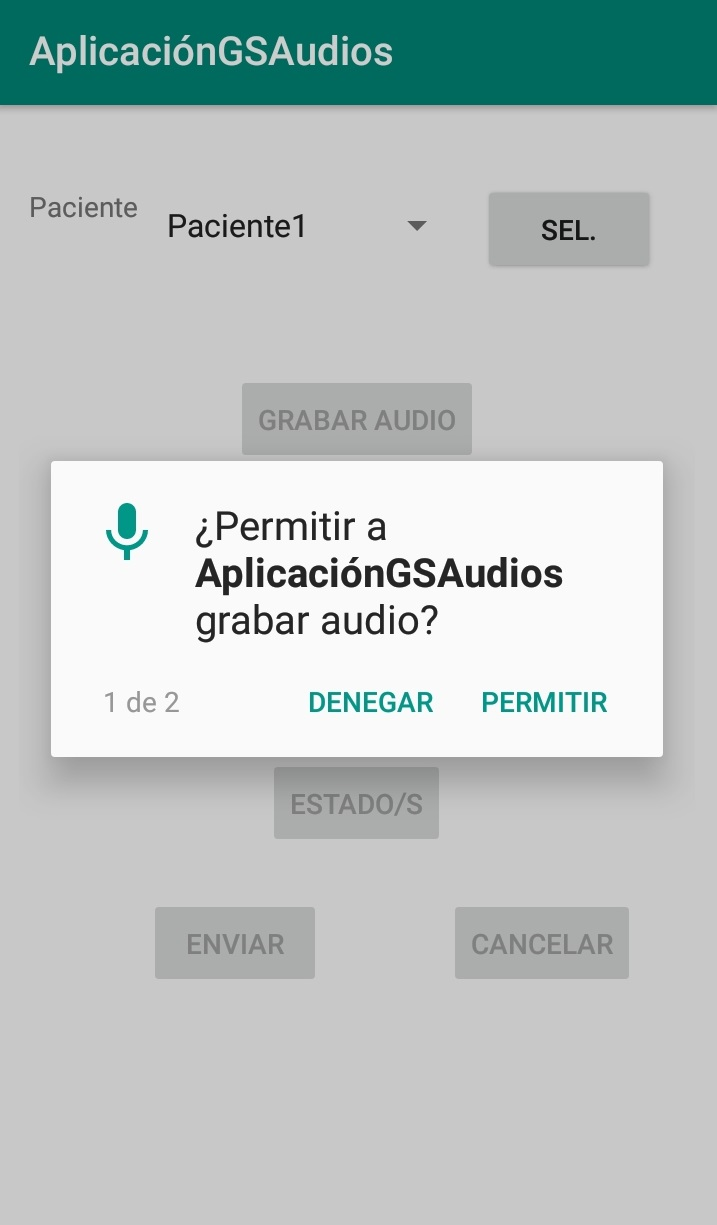
\includegraphics[scale=0.3]{gdper1}
	\caption{Petición de permisos para la grabación de audio en la aplicación de recogida de datos.}
	\label{fig:gdper1}
\end{figure}

\begin{figure}[H]
	\centering
	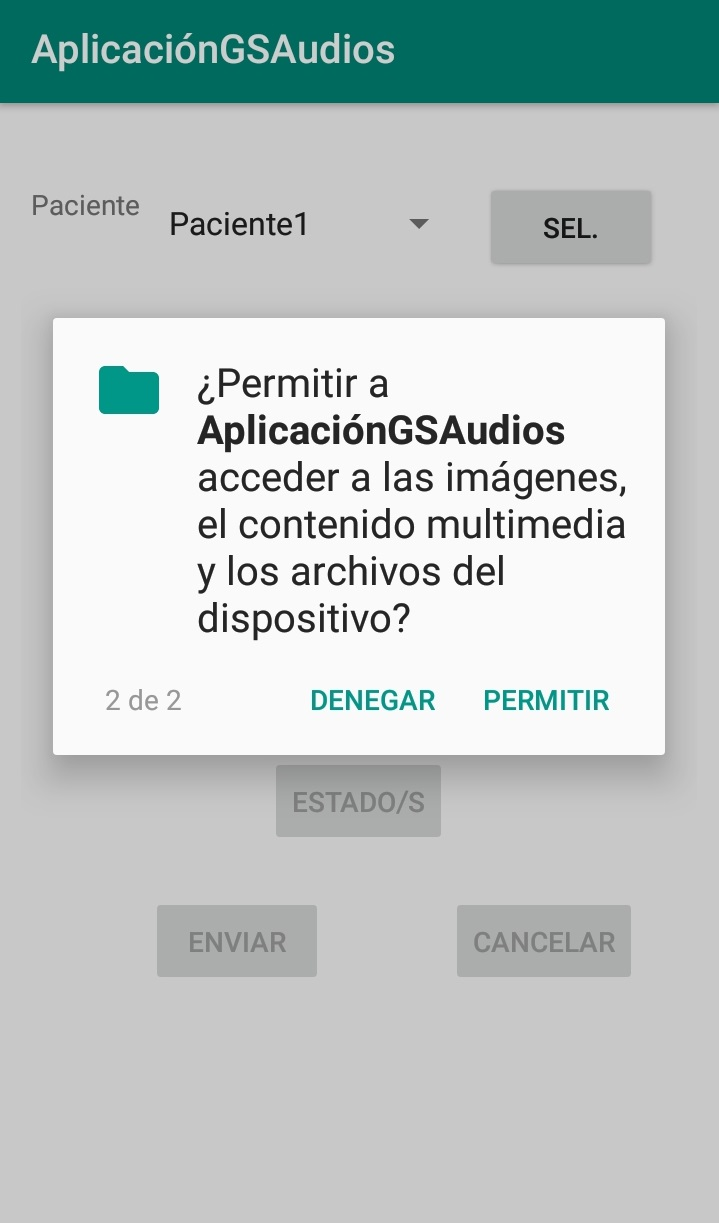
\includegraphics[scale=0.3]{gdper2}
	\caption{Petición de permisos para el acceso al almacenamiento multimedia en la aplicación de recogida de datos.}
	\label{fig:gdper2}
\end{figure}

Después de aceptar los permisos tendremos acceso al menú principal de la aplicación, como se puede ver en la figura~\ref{fig:mpgd}, en la parte superior de este, se puede ver la selección del paciente sobre el cual vamos a realizar la grabación.

\begin{figure}[h]
	\centering
	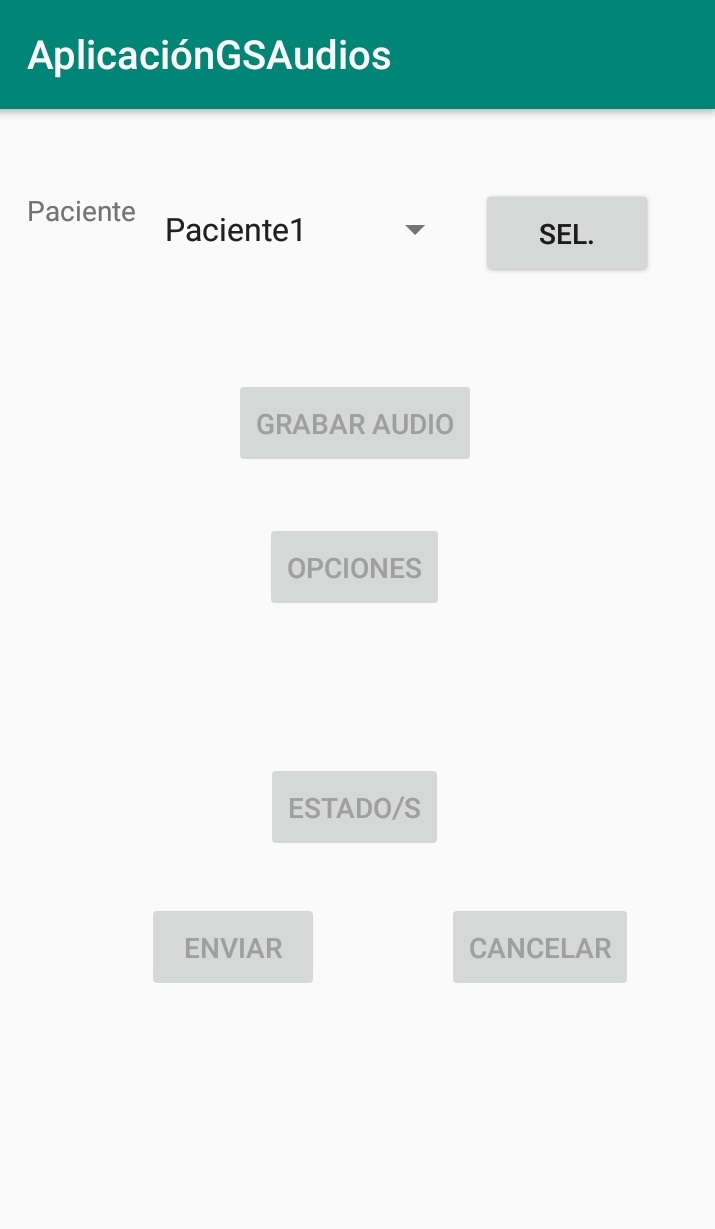
\includegraphics[scale=0.3]{mpgd}
	\caption{Menú principal de la aplicación para la recogida de datos.}
	\label{fig:mpgd}
\end{figure}

Tras haber seleccionado al paciente sobre el cual se va a recoger los datos debemos confirmar la selección del paciente pulsando el botón \textit{Sel.} (Seleccionar). Tras pulsar el botón \textit{Sel.} se nos habilitará el botón \textit{Grabar Audio}, en todo momento desde la pantalla del menú principal podremos cancelar la grabación y la selección del paciente pulsando el botón \textit{Cancelar}, como se puede ver en la figura~\ref{fig:mp2gd}.

\begin{figure}[H]
	\centering
	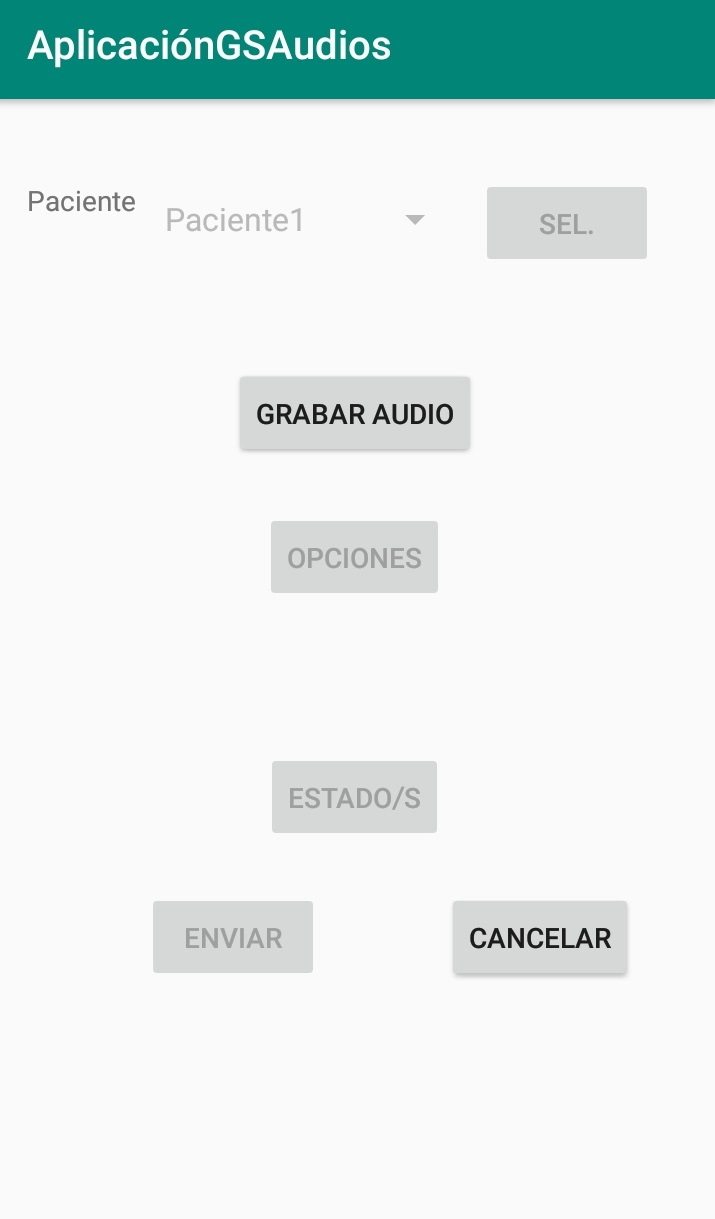
\includegraphics[scale=0.3]{mp2gd}
	\caption{Paciente seleccionado, \textit{Grabar Audio} habilitado.}
	\label{fig:mp2gd}
\end{figure}

Cuando pulsamos el botón \textit{Grabar Audio} se abrirá una nueva pantalla donde podremos grabar el audio correspondiente, como se puede ver en la figura~\ref{fig:gagd}.

\begin{figure}[H]
	\centering
	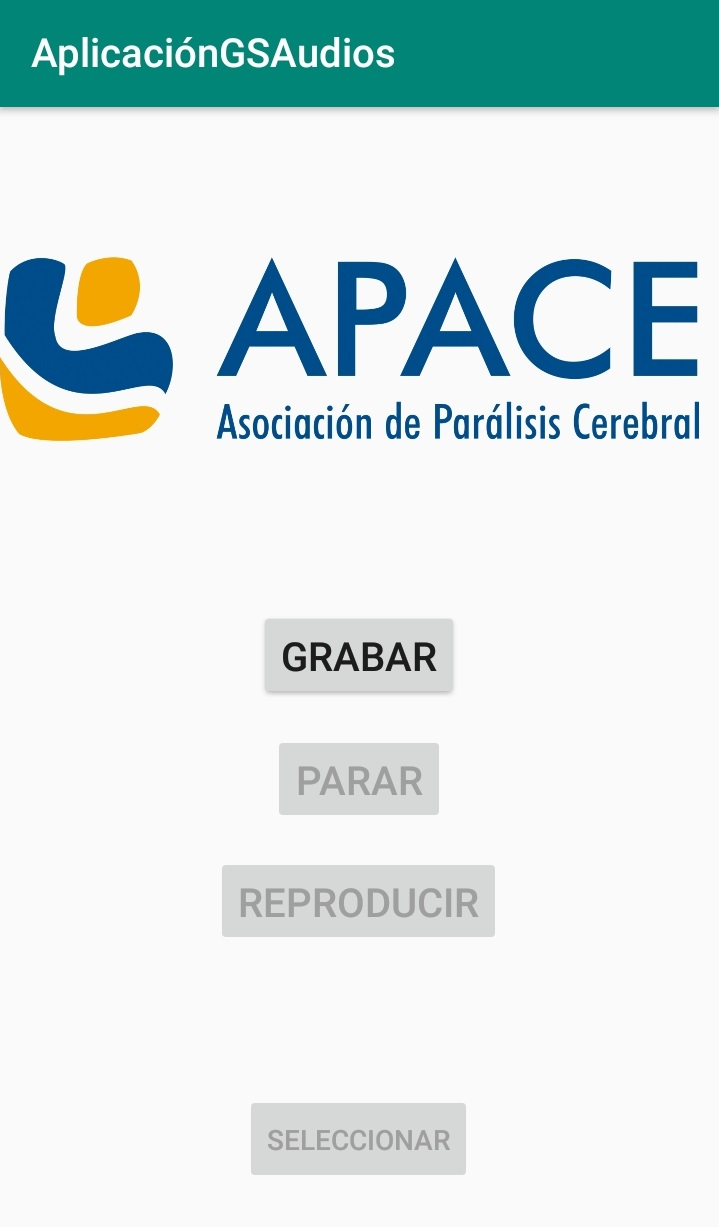
\includegraphics[scale=0.3]{gagd}
	\caption{Pantalla de Grabación de Audios.}
	\label{fig:gagd}
\end{figure}

Como se puede observar esta pantalla tiene 4 botones, pero nada más abrir la pantalla solo tenemos habilitado el botón de \textit{Grabar} que su función es comenzar a grabar el audio una vez lo pulsemos. Una vez pulsado se deshabilitará (para no poder pulsar \textit{Grabar} dos veces) y se habilitará el botón \textit{Parar}, como se puede ver en la figura~\ref{fig:ga2gd}.

\begin{figure}[htb]
	\centering
	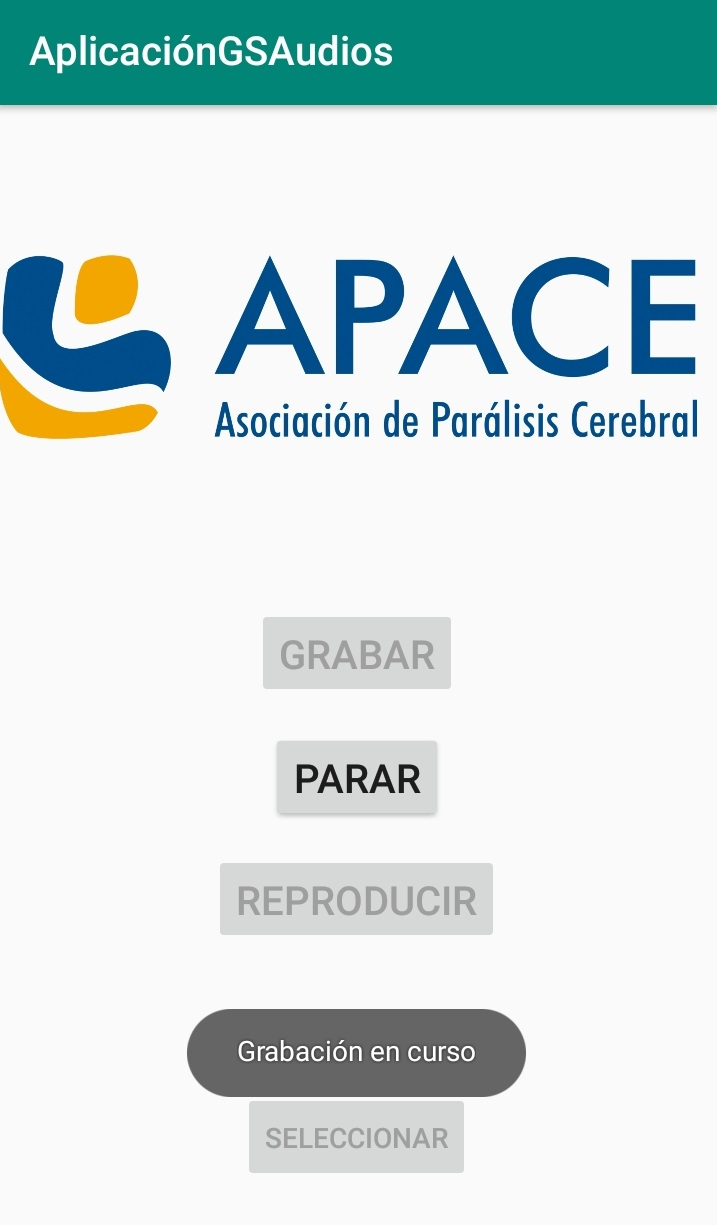
\includegraphics[scale=0.3]{ga2gd}
	\caption{Pulsamos el botón \textit{Grabar}.}
	\label{fig:ga2gd}
\end{figure}

Si pulsamos el botón \textit{Parar} se parará la grabación que habíamos comenzado, además, se habilitarán los botones de \textit{Reproducir} que nos permite reproducir el audio que se acaba de grabar, el botón \textit{Seleccionar} que nos permite seleccionar el audio y volver al menú principal y el botón \textit{Grabar} que nos permite eliminar la grabación actual y comenzar de nuevo una grabación. La interfaz tras pulsar el botón \textit{Parar} se puede ver en la figura~\ref{fig:ga3gd}.

\begin{figure}[H]
	\centering
	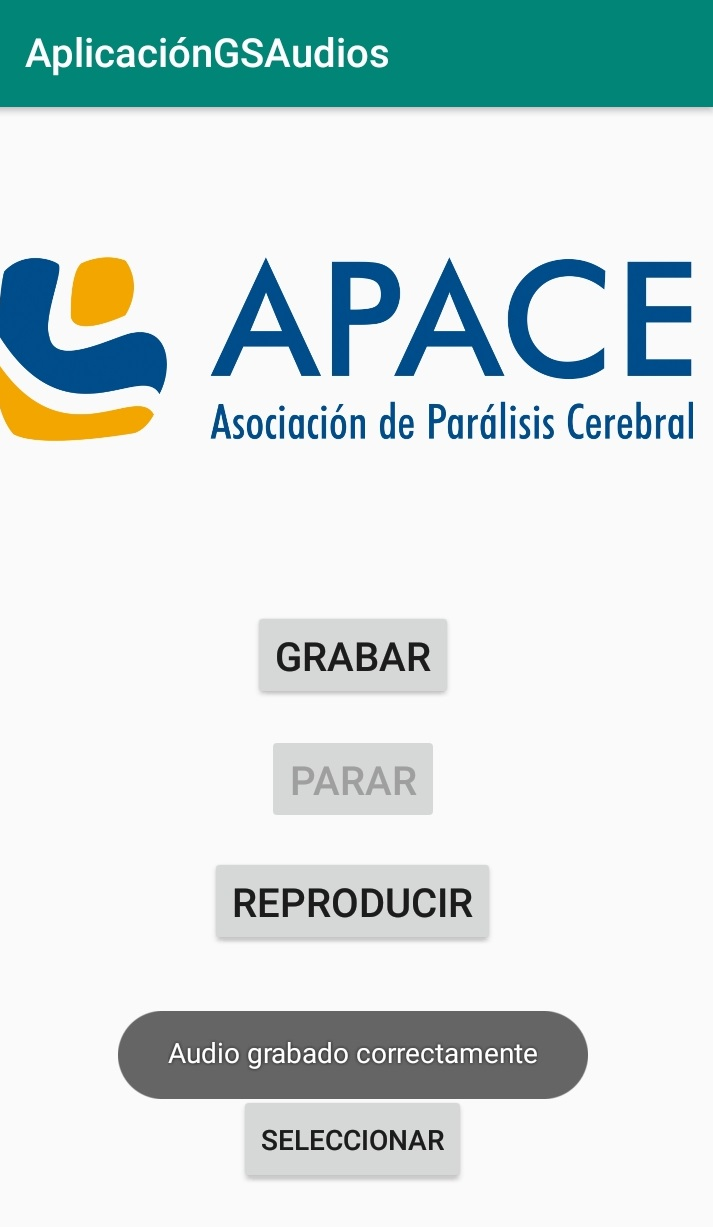
\includegraphics[scale=0.3]{ga3gd}
	\caption{Pulsamos el botón \textit{Parar}.}
	\label{fig:ga3gd}
\end{figure}

Es importante que si se quiere seleccionar el audio se pulse el botón \textit{Seleccionar} tras grabar el audio, ya que si volvemos al menú principal con el botón de ir atrás propio del móvil no se habilitará la siguiente pantalla, la pantalla de las Opciones. El menú principal tras pulsar el botón \textit{Seleccionar} se muestra en la figura~\ref{fig:mp3gd}

\begin{figure}
	\centering
	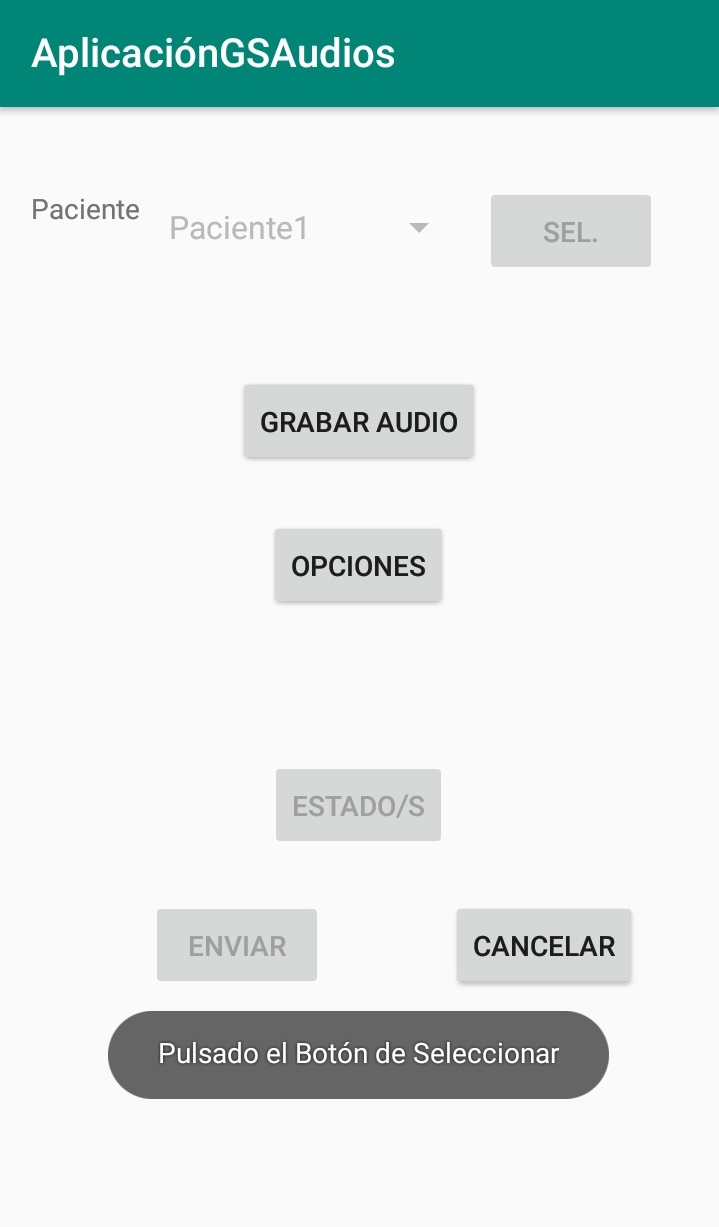
\includegraphics[scale=0.3]{mp3gd}
	\caption{Menú principal tras pulsar el botón \textit{Seleccionar}.}
	\label{fig:mp3gd}
\end{figure}

Como podemos ver, tras pulsar el botón de \textit{Seleccionar} en la pantalla de Grabación de Audio nos dirige hacia la pantalla del menú principal con el botón \textit{Opciones} habilitado, si le pulsamos iremos a la pantalla de Opciones donde podremos seleccionar las opciones adicionales, esta pantalla la podemos ver en la figura~\ref{fig:opgd}.

\begin{figure}[H]
	\centering
	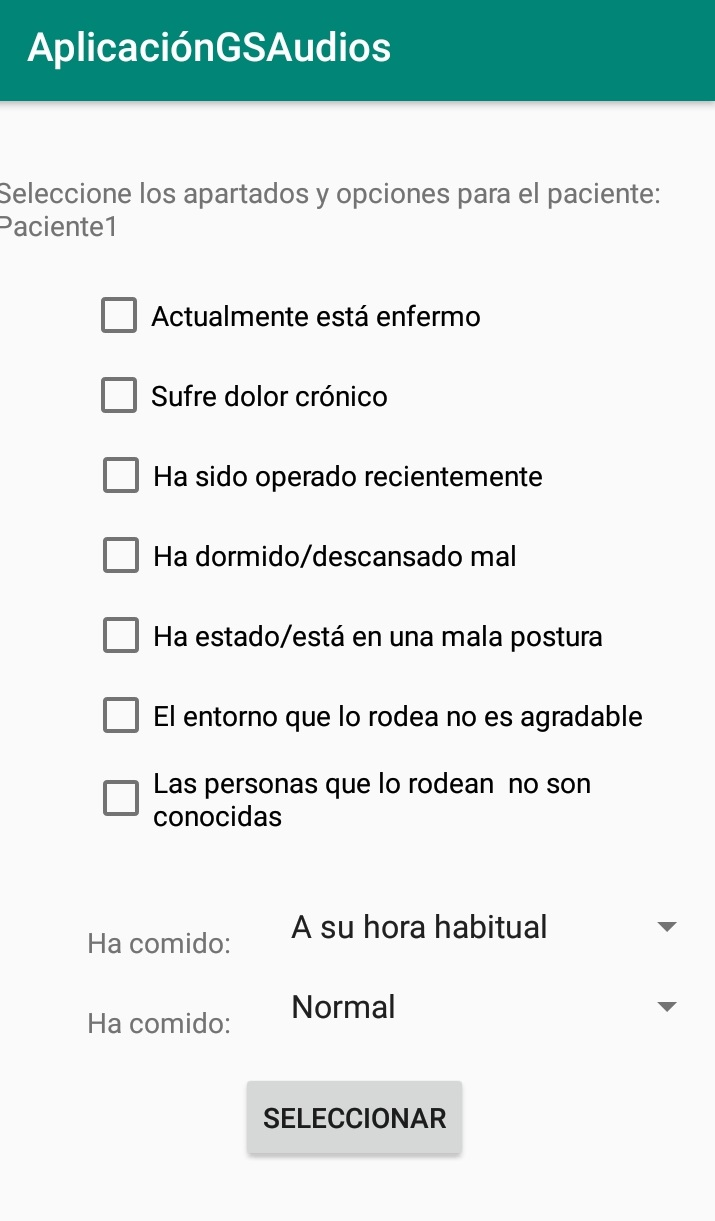
\includegraphics[scale=0.3]{opgd}
	\caption{Pantalla para seleccionar las opciones adicionales.}
	\label{fig:opgd}
\end{figure}

Una vez hayamos rellenado el formulario tenemos que pulsar el botón \textit{Seleccionar} que nos volverá a la pantalla del menú principal. Como pasaba en la pantalla anterior, debemos volver al menú principal a partir de el botón \textit{Seleccionar}, ya que sino no se desbloqueará el botón de \textit{Estado} en el menú principal. El menú principal tras pulsar el botón \textit{Seleccionar} en la pantalla de las opciones se puede ver en la figura~\ref{fig:mp4gd}.

\begin{figure}
	\centering
	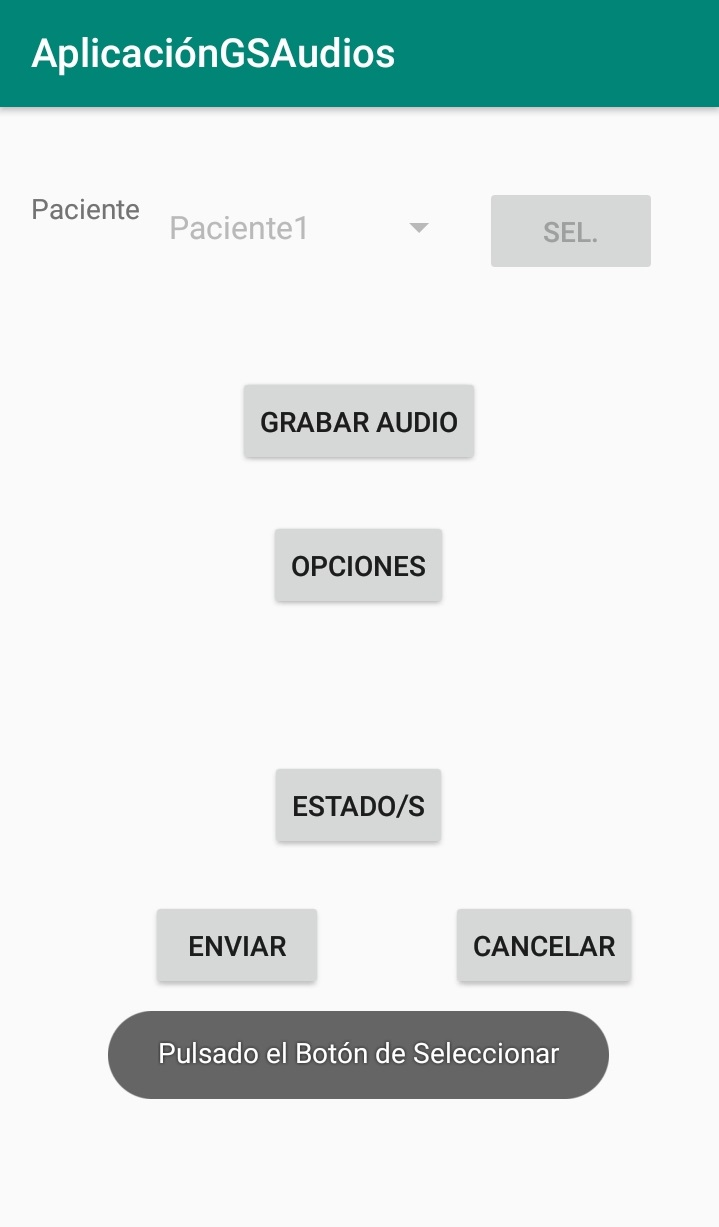
\includegraphics[scale=0.3]{mp4gd}
	\caption{Menú principal tras pulsar el botón \textit{Seleccionar} en la pantalla de opciones.}
	\label{fig:mp4gd}
\end{figure}

Como podemos observar, al pulsar el botón \textit{Seleccionar} en la pantalla de Opciones nos redirige al menú principal con el botón \textit{Estado/s} habilitado. Si pulsamos este botón \textit{Estado/s} nos llevará a la pantalla de selección de estados donde podremos elegir la emoción o respuesta que creemos que tiene el paciente (se puede seleccionar más de uno, pero de distintas columnas, es decir, se puede seleccionar por ejemplo dolor y hambre, pero no se puede seleccionar dolor y sí). Esta pantalla se puede ver en la figura~\ref{fig:ergd}.

\begin{figure}[H]
	\centering
	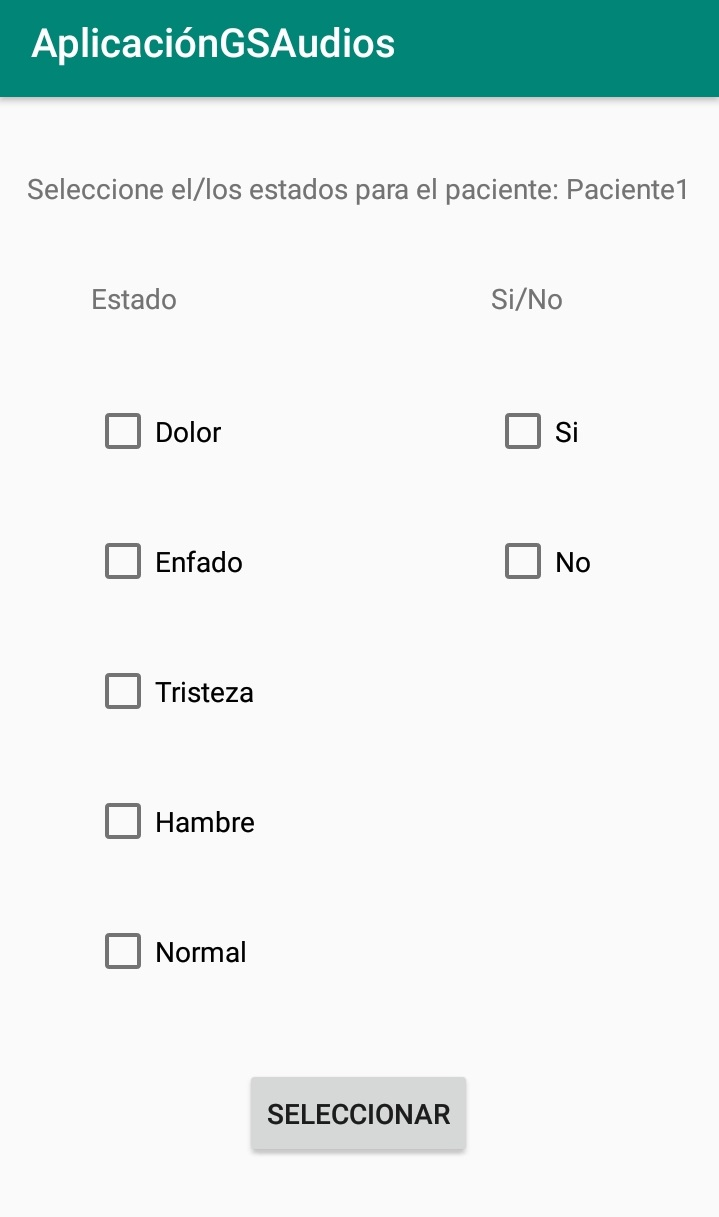
\includegraphics[scale=0.3]{ergd}
	\caption{Pantalla de selección de emociones o respuesta.}
	\label{fig:ergd}
\end{figure}

Como podemos observar en esta pantalla nos permite seleccionar una o más emociones de la primera columna o la respuestas sí o no en la segunda. Con el botón \textit{Seleccionar} guardaremos y volveremos al menú principal, si y solo si hemos cumplido las siguientes reglas en la selección de estados:
\begin{itemize}
	\item Hemos seleccionado elemento/s de solo una de las dos columnas.
	\item Hemos seleccionado algún elemento.
	\item No hemos seleccionado sí y no a la vez.
\end{itemize}

Si no se cumplen todas estas reglas aparecerá un mensaje informativo, y no se nos permitirá volver al menú principal, como se puede ver en la figura~\ref{fig:er2gd}.
\begin{figure}
	\centering
	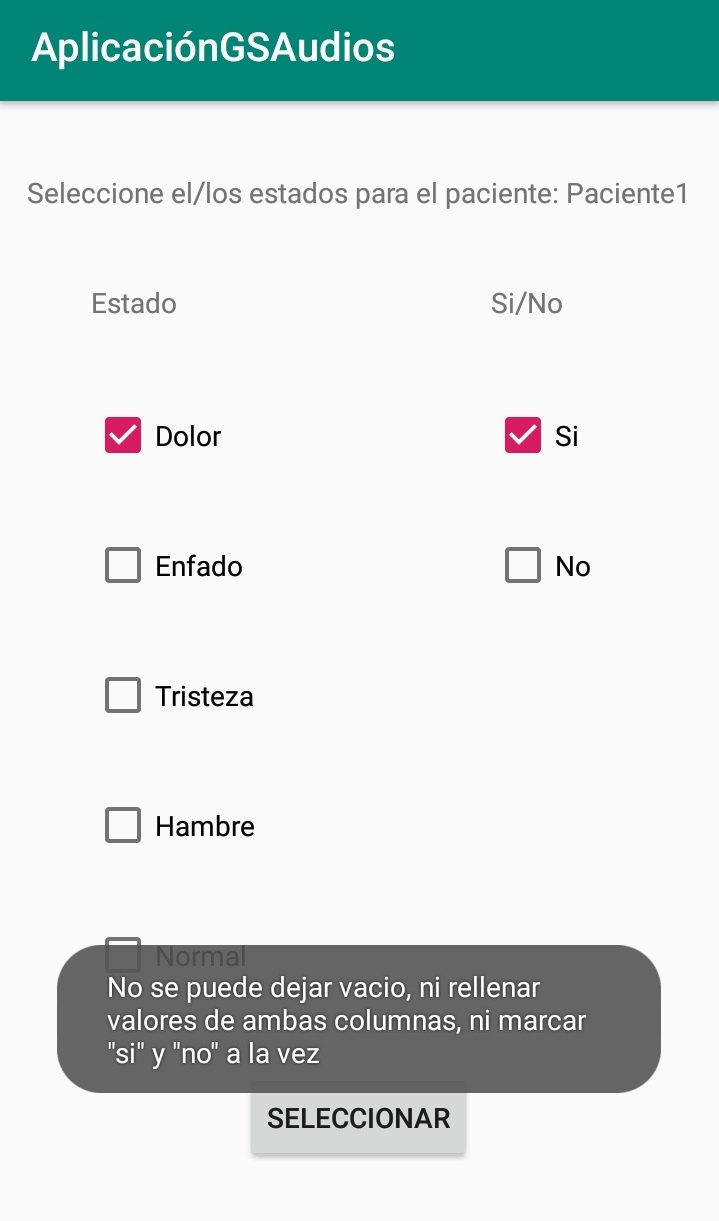
\includegraphics[scale=0.3]{er2gd}
	\caption{Mensaje informativo con el error.}
	\label{fig:er2gd}
\end{figure}
Si por el contrario, no ha ocurrido ningún error al pulsar el botón \textit{Seleccionar} iremos al menú principal teniendo ya todo completado para poder enviar.

Desde el menú principal, tras volver de la pantalla de Estado/s dando al botón \textit{Seleccionar} se nos habrá habilitado el botón de \textit{Enviar} que nos permite comprimir nuestros archivos y enviarlos para la investigación, siempre que haya conexión a Internet, si no tienes conexión a Internet le saldrá el siguiente mensaje (podrá volverse a conectar a Internet y volver a pulsar el botón de \textit{Enviar}), como se puede ver en la figura~\ref{fig:mp5gd}.

\begin{figure}[H]
	\centering
	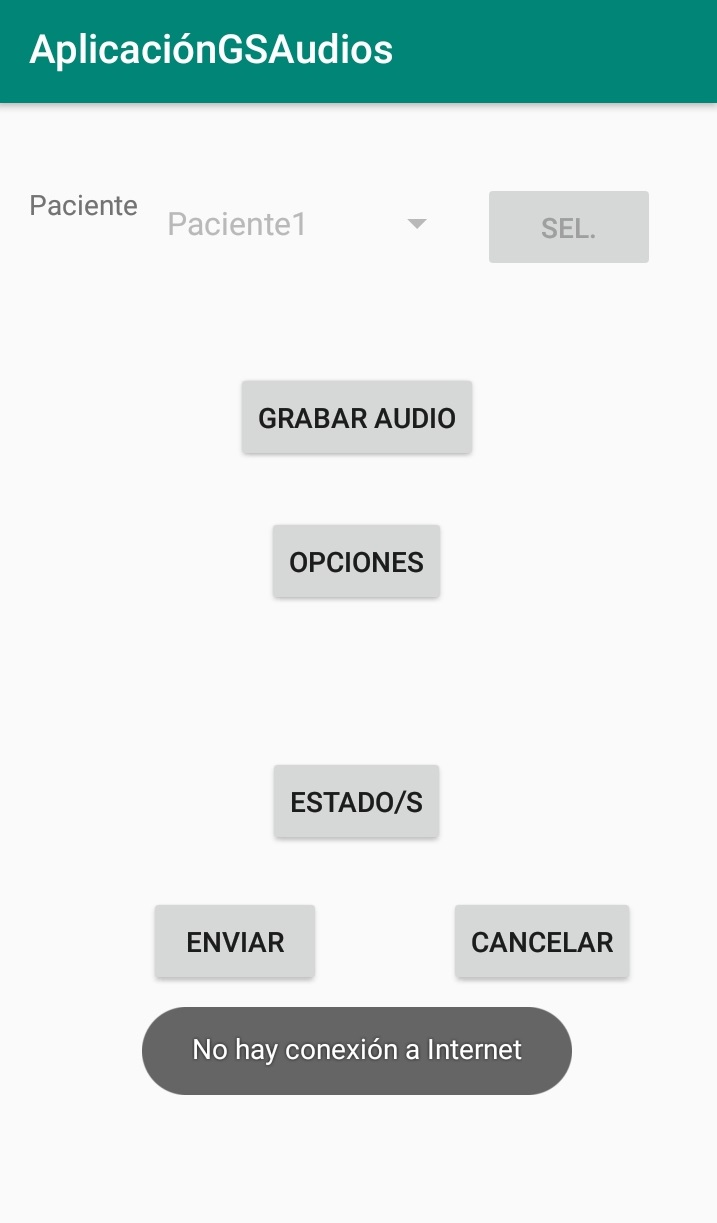
\includegraphics[scale=0.3]{mp5gd}
	\caption{Mensaje de error al intentar enviar sin conexión a Internet.}
	\label{fig:mp5gd}
\end{figure}

Si tenemos conexión el comprimido se generará y se enviará para su posterior investigación.

Cabe destacar que en cualquier momento se puede volver a ir a una pantalla (Grabar Audios, Opciones y Estado/s) una vez visitada, para observar lo que se tiene marcado o para modificarlo.
\newpage
\section{Aplicación para la interpretación}
\subsection{Uso}
Esta aplicación sirve para interpretar las emociones y las respuestas de las personas con parálisis cerebral de las cuales se han obtenido los datos suficientes como para poder haber creado los algoritmos correspondientes y necesarios. Si el paciente al que desea interpretar no está en la lista de pacientes disponibles ha de seguir grabando datos válidos para ese paciente.
\subsection{Requisitos}
El requisito principal es contar con un dispositivo \textit{smartphone Android} actualizado con una versión \textit{Android} 6.0 o superior y conexión a directa vía \textit{Wi-Fi} al servidor.
\subsubsection{Instalación}
Para poder instalar la aplicación el único requisito que se necesita es conexión a Internet para poder descargarse la aplicación.
\subsubsection{Ejecución}
Para la ejecución de la aplicación se requiere que esta esté instalada, que se acepten los permisos de grabación de audio y de escritura que se preguntan al principio de la ejecución y conexión directa con el servidor.
\subsection{Instalación}
La instalación del prototipo es sencilla, solo hay que descargar el archivo \textit{apk} desde donde se haya sido suministrado (correo, \textit{WhatsApp}, \textit{GitHub}) y realizar los ajustes necesarios para poder descargarla al ser una aplicación ajena a \textit{Play Store}.

Estos ajustes adicionales consisten simplemente aceptar que se descargue esta aplicación exterior a \textit{Play Store}.

Una vez descargada la \textit{apk} la aplicación aparecerá en su menú de aplicaciones instaladas con el nombre de AVC, como se puede ver en la figura~\ref{fig:logoavc}.

\begin{figure}[htp]
	\centering
	
\includegraphics[scale=0.6]{logoavc}
	\caption{Logotipo y nombre de la aplicación de interpretación, AVC.}
	\label{fig:logoavc}
\end{figure}

\subsection{Ejecución}
Para la ejecución solo tenemos que seleccionar el logotipo anteriormente mostrado. En la primera ejecución que hagamos del prototipo nos saldrá el siguiente diálogo para pedirnos permisos para poder usar tanto el sistema de grabación de audio como para poder almacenar archivos, debemos dar permisos a ambos pulsando en la opción \textit{Permitir}, es muy importante aceptar estos permisos ya que sino la aplicación se cerrará en la primera vez que queramos grabar un audio. En cualquier caso, si por algún error se ha denegado los permisos y la aplicación se ha cerrado se puede volver a abrir y nos volverá a pedir aceptar los permisos. La forma en la que se piden estos permisos se puede ver en las figuras~\ref{fig:avcper1} y ~\ref{fig:avcper2}.

\begin{figure}[htp]
	\centering
	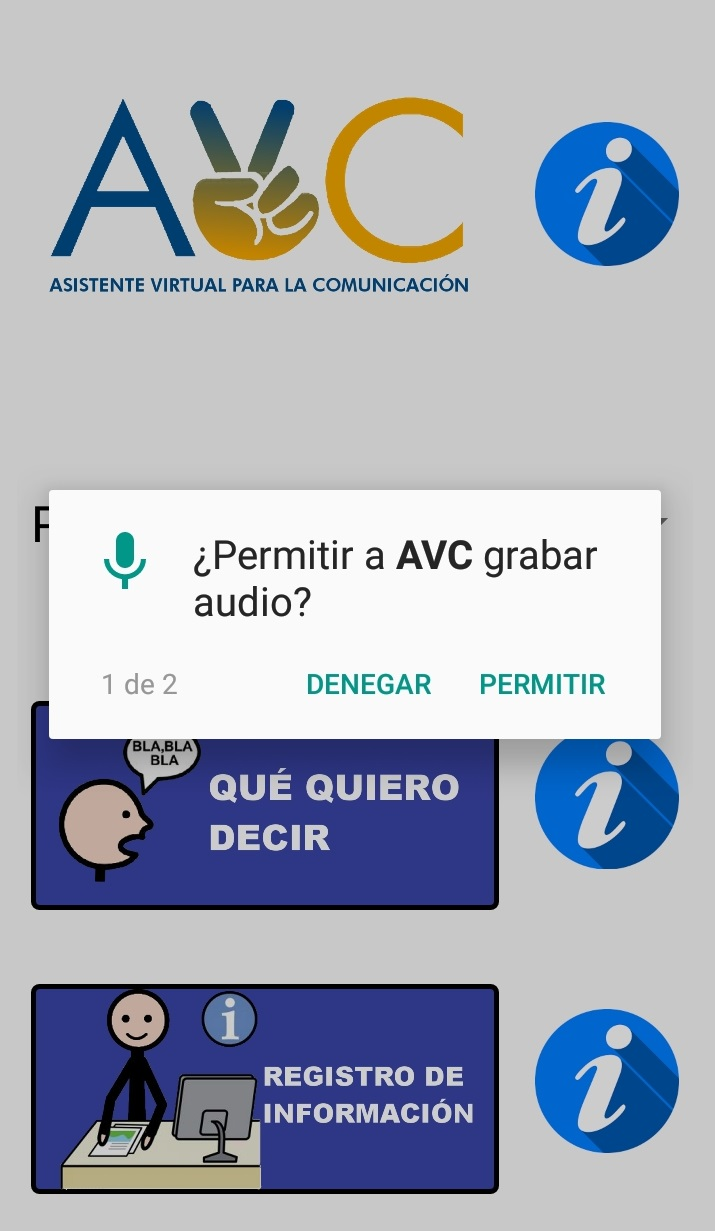
\includegraphics[scale=0.3]{avcper1}
	\caption{Permisos de grabación de audio en AVC.}
	\label{fig:avcper1}
\end{figure}

\begin{figure}[htp]
	\centering
	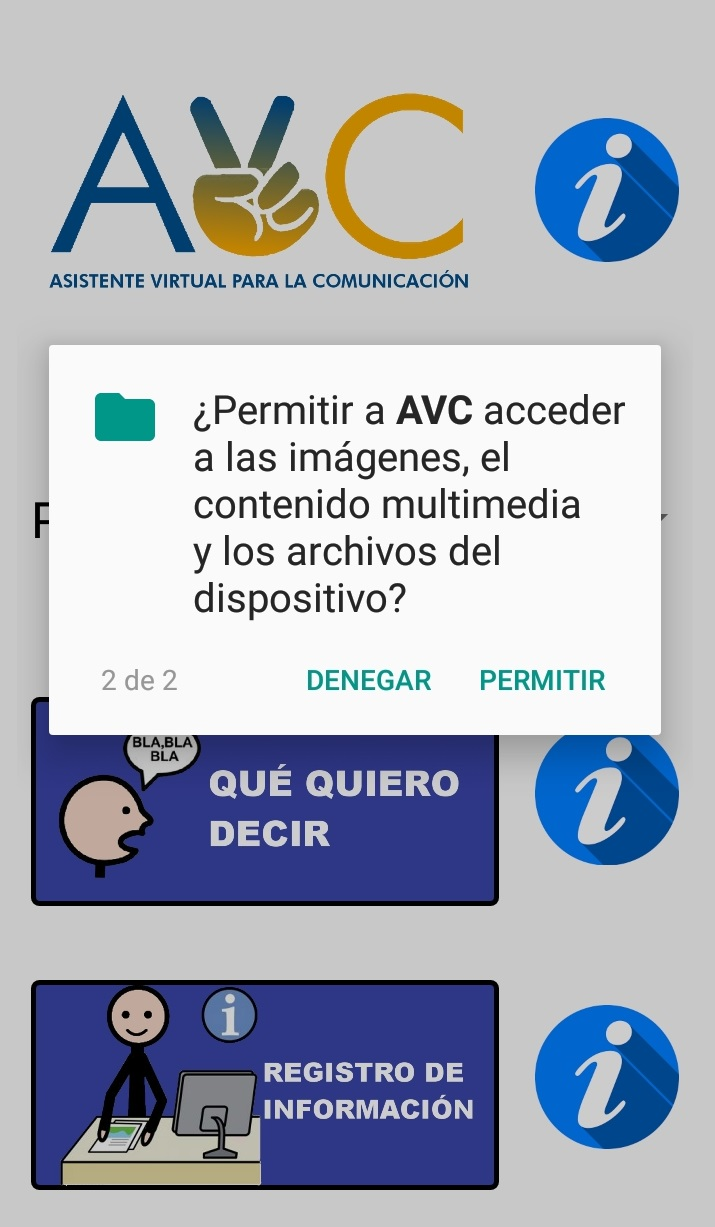
\includegraphics[scale=0.3]{avcper2}
	\caption{Permisos para el acceso a multimedia en AVC.}
	\label{fig:avcper2}
\end{figure}

Después de aceptar los permisos tendremos acceso al menú principal de la aplicación, aquí podremos seleccionar el paciente con el cual queremos trabajar (el último paciente que se seleccionó antes de cerrar la aplicación será el paciente que aparezca como seleccionado cuando volvamos a ejecutar la aplicación). El menú principal de la aplicación se puede ver en la figura~\ref{fig:mpavc}.

\begin{figure}[H]
	\centering
	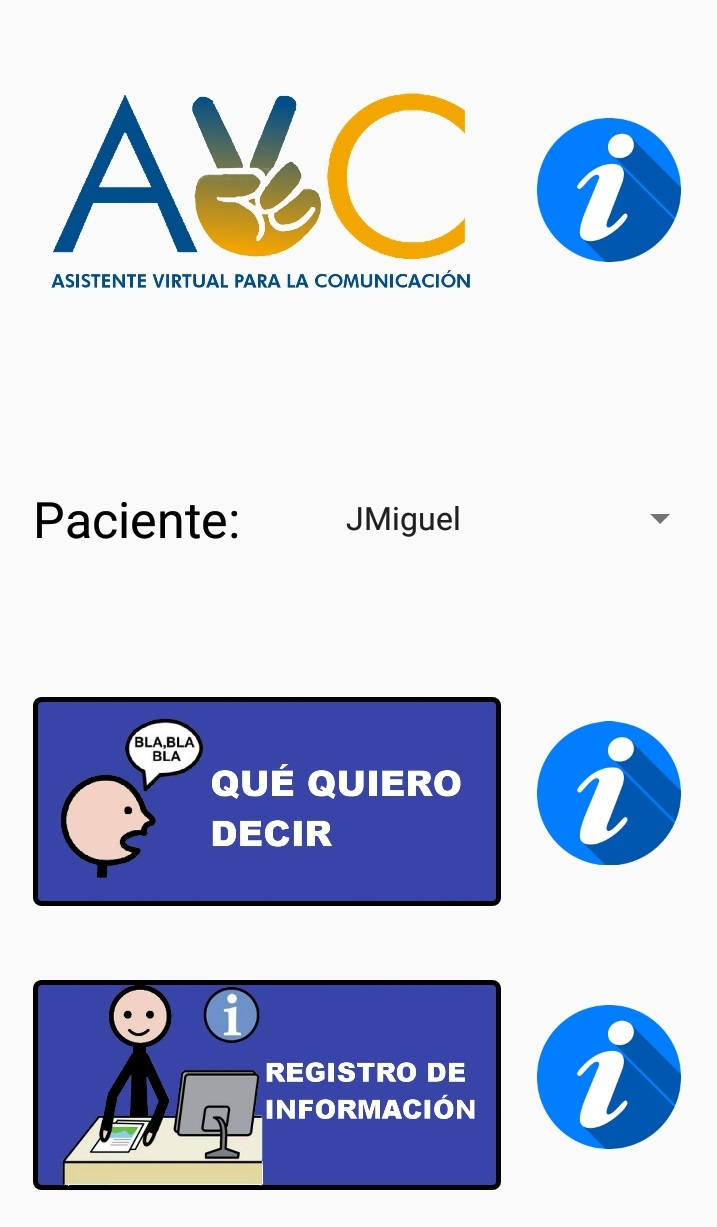
\includegraphics[scale=0.3]{mpavc}
	\caption{Menú principal de la aplicación AVC.}
	\label{fig:mpavc}
\end{figure}

Tras haber seleccionado a nuestro paciente podemos hacer dos cosas diferentes, o podemos modificar las opciones adicionales relacionadas con ese paciente o podemos interpretar una emoción o una respuesta.

Si queremos modificar o ver las opciones adicionales del paciente seleccionado tenemos que pulsar el botón de \textit{Registro de Información}, que nos llevará a la pantalla donde podremos ver las opciones guardadas para ese paciente, como se puede ver en la figura~\ref{fig:opcavc}.

\begin{figure}[htp]
	\centering
	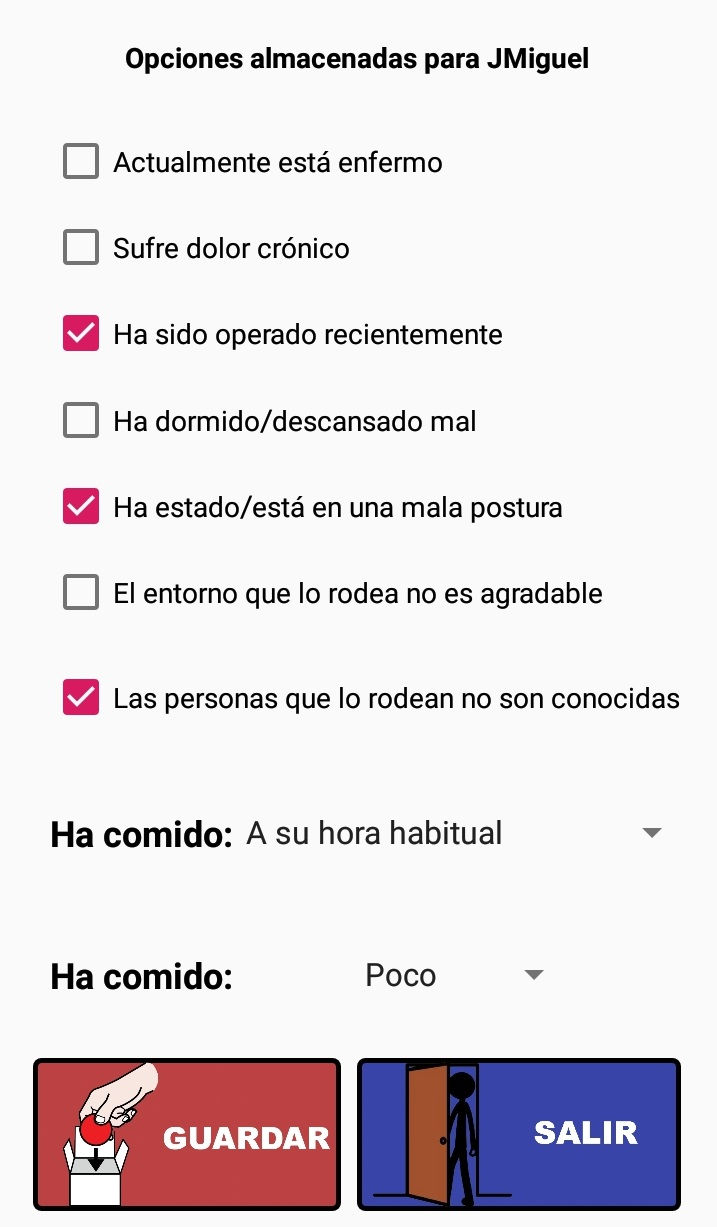
\includegraphics[scale=0.3]{opcavc}
	\caption{Pantalla con las opciones cargadas del paciente seleccionado.}
	\label{fig:opcavc}
\end{figure}

Al cargar la pantalla se verán las opciones almacenadas para el paciente seleccionado, aquí podemos salir si no queremos modificar ninguna opción pulsando el botón \textit{Salir} o podemos modificar alguna de las opciones, entonces el botón \textit{Guardar} se pondrá en azul por lo que estaría disponible, y pulsándolo haría que se guarden las opciones. El cambio en el botón \textit{Guardar} se puede observar en la siguiente figura~\ref{fig:opc2avc}.

\begin{figure}[htp]
	\centering
	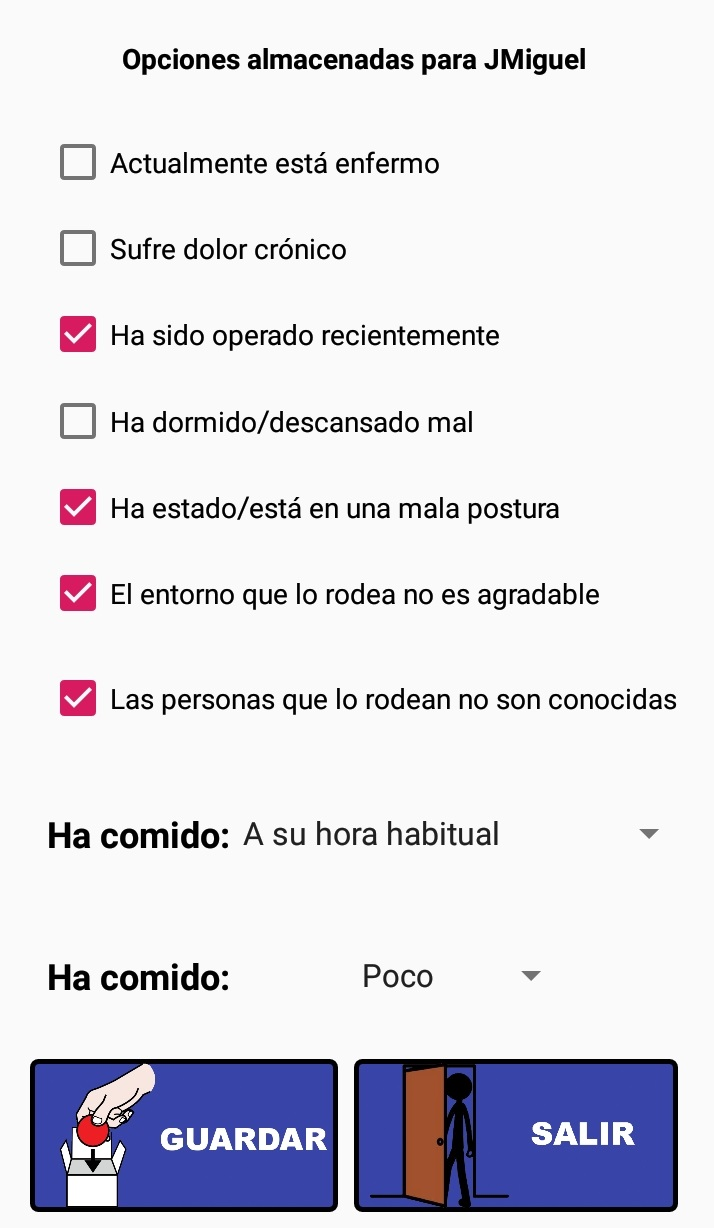
\includegraphics[scale=0.3]{opc2avc}
	\caption{Botón \textit{Guardar} habilitado.}
	\label{fig:opc2avc}
\end{figure}

Una vez pulsados el botón \textit{Salir} o \textit{Guardar} volveremos a la pantalla principal.

Si por el contrario lo que queremos es interpretar una emoción o una respuesta tenemos que pulsar en el menú principal \textit{Qué quiero decir}, este nos llevará a una nueva pantalla, la pantalla de selección de interpretación, que se puede ver en la figura~\ref{fig:interpavc}.

\begin{figure}[htp]
	\centering
	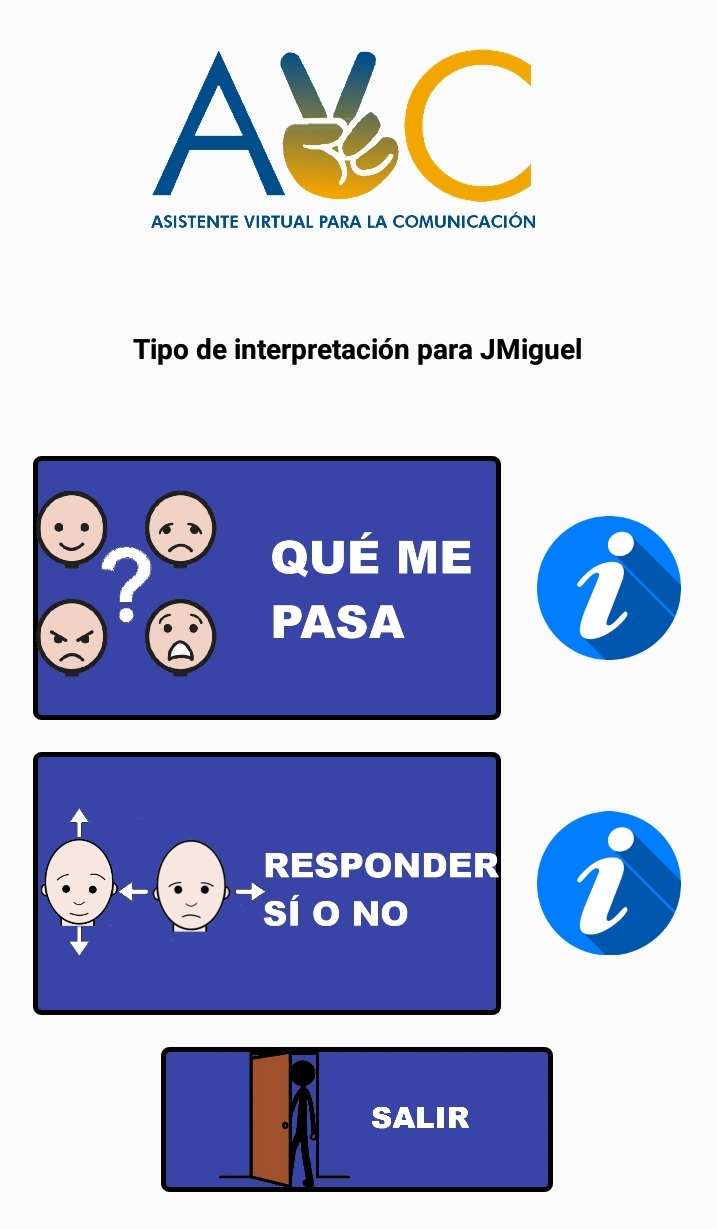
\includegraphics[scale=0.3]{interpavc}
	\caption{Pantalla de selección del tipo de interpretación.}
	\label{fig:interpavc}
\end{figure}

En esta pantalla podemos pulsar el botón \textit{Salir} que nos llevaría de nuevo al menú principal, o podemos pulsar en los botones de \textit{Qué me pasa} si queremos interpretar una emoción, o \textit{Responder sí o no} si queremos interpretar una respuesta.

Cualquier tipo de interpretación que pulsemos nos llevará a la pantalla de grabación del audio, que se puede ver en la figura~\ref{fig:gaavc}.

\begin{figure}[htp]
	\centering
	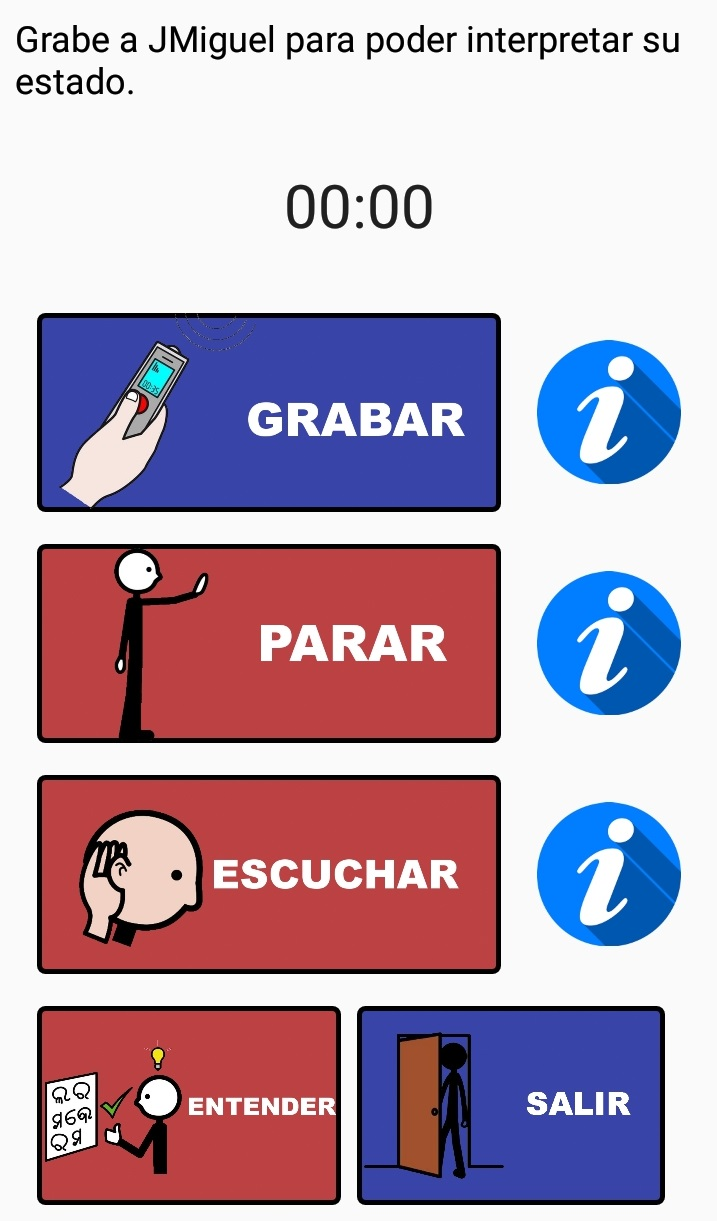
\includegraphics[scale=0.3]{gaavc}
	\caption{Pantalla de grabación del audio.}
	\label{fig:gaavc}
\end{figure}

En esta pantalla podemos grabar el audio que queremos interpretar. Como en el resto de las pantallas, tenemos el botón \textit{Salir} que nos devuelve a la pantalla anterior, la pantalla de selección de interpretación.

Si por el contrario queremos grabar un audio solo tenemos que pulsar el botón \textit{Grabar} para comenzar a grabar, entonces el contador empezará a sumar mostrándonos el tiempo de grabación, como se puede ver en la figura~\ref{fig:ga2avc}.

\begin{figure}[htp]
	\centering
	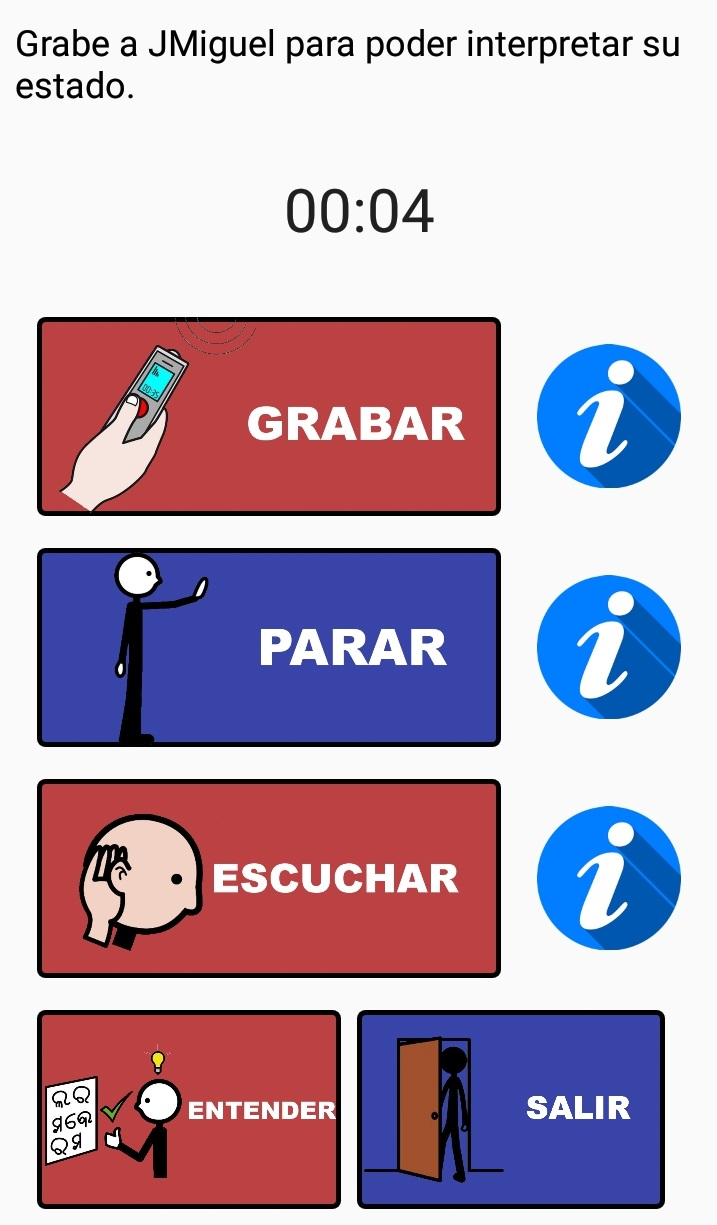
\includegraphics[scale=0.3]{ga2avc}
	\caption{Empezamos a grabar, tras pulsar \textit{Grabar}.}
	\label{fig:ga2avc}
\end{figure}

Si queremos parar de grabar entonces tenemos que pulsar el botón \textit{Parar}, entonces el audio se guardará y podremos escucharlo pulsando el botón \textit{Escuchar} o intepretarlo pulsando el botón \textit{Entender}, como se puede ver en la figura~\ref{fig:ga3avc}.

\begin{figure}[htp]
	\centering
	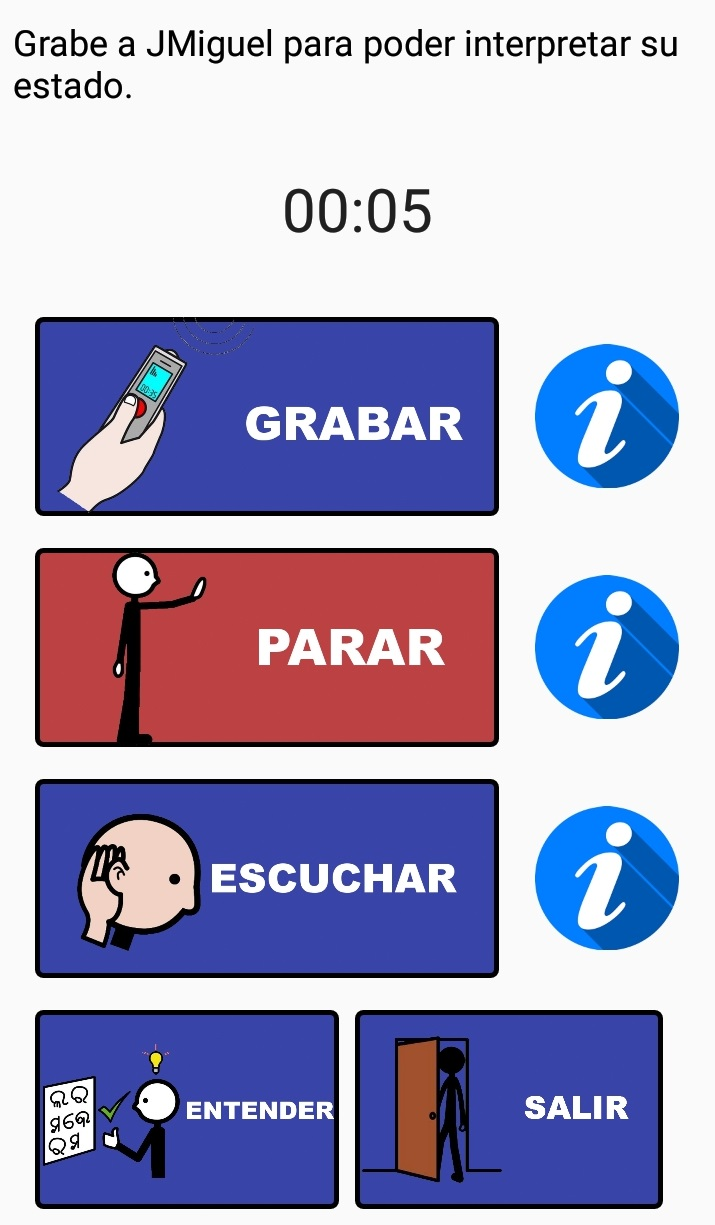
\includegraphics[scale=0.3]{ga3avc}
	\caption{Paramos la grabación, tras pulsar \textit{Parar}.}
	\label{fig:ga3avc}
\end{figure}

Una vez grabado el audio podemos volver a grabarlo pulsando de nuevo el botón \textit{Grabar}, que iniciaría de nuevo la grabación. Si por el contrario el audio es correcto y es el que queremos interpretar tenemos que pulsar en el botón \textit{Entender} que nos llevará a la pantalla donde encontraremos el resultado de la interpretación. Un ejemplo de un resultado de una interpretación se puede ver en la figura~\ref{fig:resavc}.

\begin{figure}[htp]
	\centering
	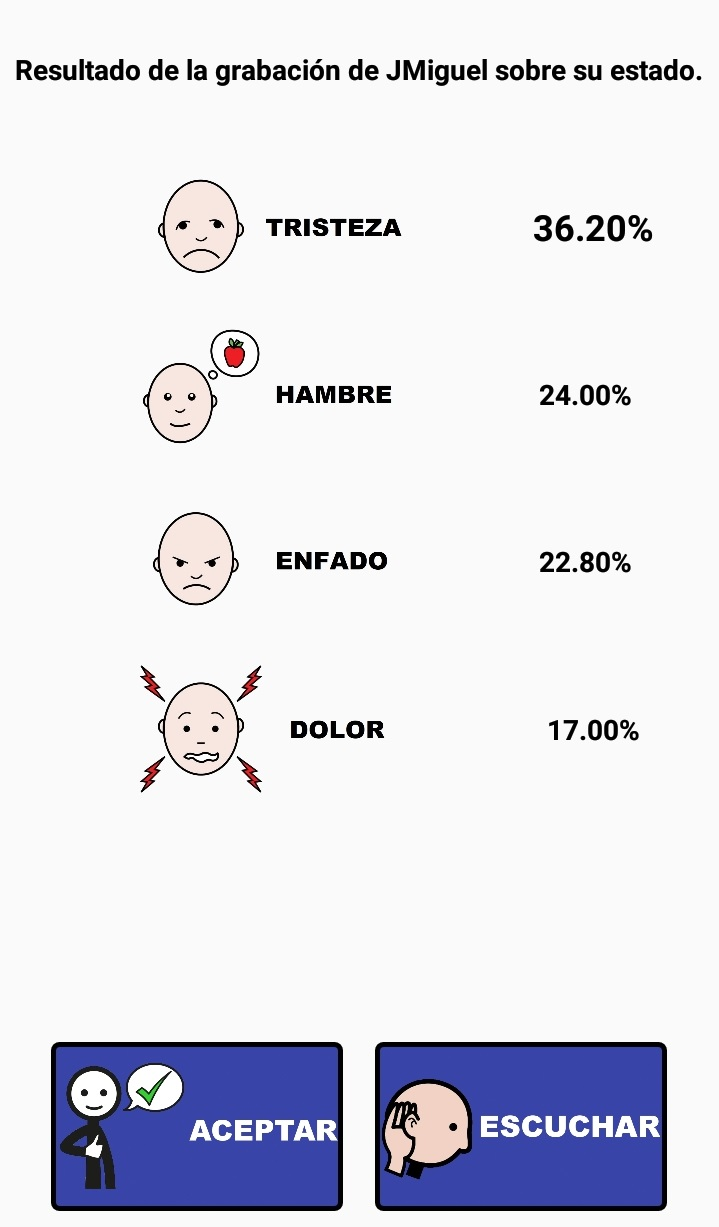
\includegraphics[scale=0.3]{resavc}
	\caption{Ejemplo de la pantalla con el resultado de una interpretación.}
	\label{fig:resavc}
\end{figure}

En esta pantalla podremos ver el resultado con porcentajes de la interpretación, siendo el que viene más arriba el resultado con mayor porcentaje. En esta pantalla podemos volver a escuchar el audio que hemos interpretado pulsando el botón \textit{Escuchar}, o podemos salir al menú principal pulsando el botón \textit{Aceptar}.

Además, a lo largo de la aplicación nos podemos encontrar con distintos botones de información a la derecha de otros botones, estos botones de información nos abren un dialogo en el cual se nos comunica vía texto en lectura fácil y por audio lo que hace el botón que tiene a la izquierda, un ejemplo de estos diálogos se puede ver en la figura~\ref{fig:diaavc}.

\begin{figure}[htp]
	\centering
	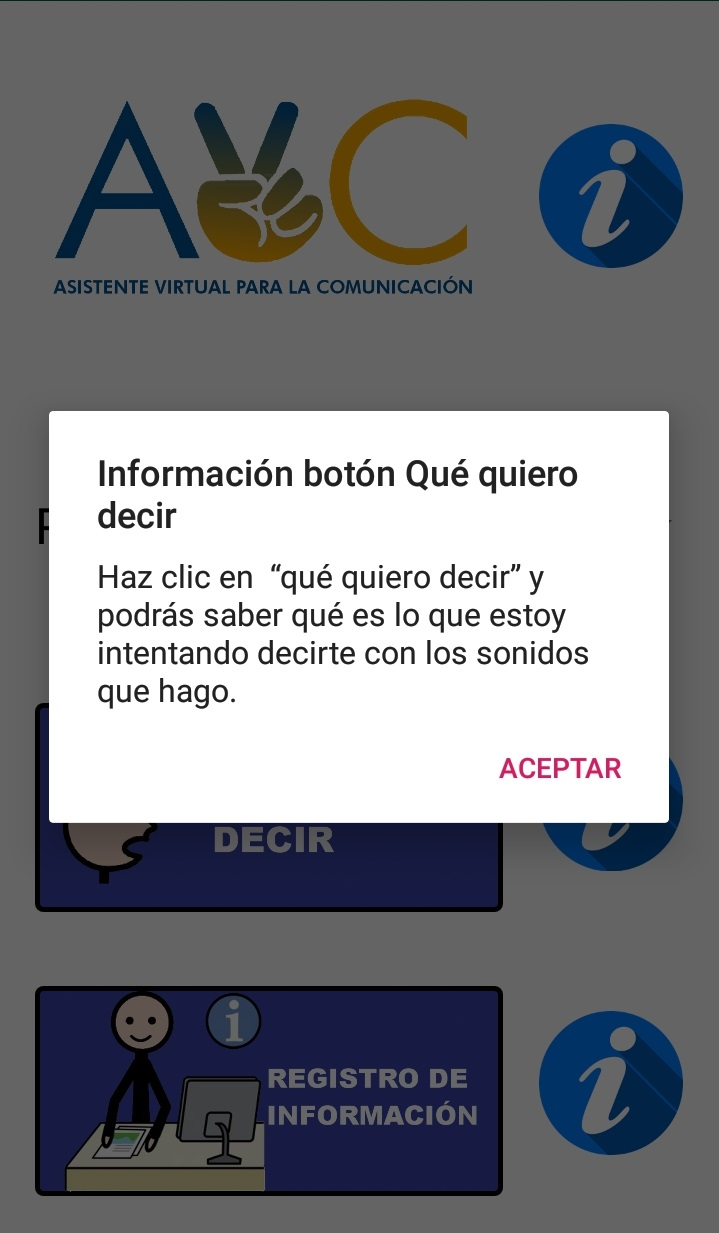
\includegraphics[scale=0.3]{dialogo}
	\caption{Ejemplo de diálogo informativo.}
	\label{fig:diaavc}
\end{figure}